\section{Theoretical Background}
%%%%%%%%%%%%%%%%%%%%%%%%%%%%%%%%%%%%%%%%%%%%%%%%%%%%%









%%%%%%%%%%%%%%%%%%%%%%%%%%%%%%%%%%%%%%%%%%%%%%%%%%%%%

\subsection{Machine Learning}
\textcite{shalevbook} describe \gls{ML} as automated learning where an algorithm gets training data as input and uses it to optimize certain parameters to find the optimal solution to a given problem. Depending on if the training data is labeled, the learning process can be divided into supervised or unsupervised learning \autocite{shalevbook}. This review focuses on supervised learning since the input data, MRI-images, are labeled with the patients official diagnosis (see Chapter \ref{Training Data}). 


%%%%%%%%%%%%%%
\subsubsection{Support Vector Machine} \label{Support Vector Machine}

\gls{svm} is among the most widely used machine learning techniques for classifying \gls{AD} \autocite{tanveerMachineLearningTechniques2020}. It is thought to have good accuracy and sensitivity (terms are described in \ref{Model Selection}) and can handle high-dimensional data well \autocite{toshkhujaevClassificationAlzheimerDisease2020}. 
\gls{svm} uses features (independent variables) as input and predicts the class (dependent variable) of an observation (set of independent variable values) \autocite{pereiraMachineLearningClassifiers2009}. For example, \textcite{burges1998tutorial} illustrate this with a tree recognition problem where each observation would consist of a feature vector (e.g. pixel values) and a class (e.g. is the observation a tree or not: 1 or -1). \gls{svm} then uses these observations to adjust the parameters to solve the binary classification task in an optimal manner. For example, with \gls{mri}-images the features used as input can be voxel-based \autocite{tohkaComparisonFeatureSelection2016}, meaning the input comes as vectors with voxel intensity values of the image \autocite{ebrahimighahnaviehDeepLearningDetect2020}. 
Essentially, as described in \textcite{bishop2006pattern}, \gls{svm} achieves the classification task through learning the optimal hyperplane that separates the two classes using maximum margin principle.  Put simply, a hyperplane can be a line, plane or some other flat subspace depending on the dimensional space it is formed in and margin being the perpendicular distance between the hyperplane and the nearest observation \autocite{introtostat}. \textcite{bishop2006pattern} states, that to help with generalization (see \ref{bias-variance}) missclassifications of some data points are allowed, which relaxes the hard margin and hence are called soft margin. To find the optimal amount of missclassifications, a tuning parameter that essentially controls the bias-variance trade-off (see \ref{bias-variance}) is chosen via cross-validation (see \ref{Model Selection}) \autocite{introtostat}.
Therefore, \gls{svm}'s goal becomes to maximize the margin while softly penalizing missclassifications. 


\gls{svm} can be linear or non-linear depending if the training data is linear separable or not \autocite{burges1998tutorial}. Non-linear \gls{svm} follow the idea of mapping an input vector into a feature space with a higher dimension where the input becomes linear separable \autocite{natureofstat}. To save computational costs, a kernel function is used  to avoid explicitly transforming, or mapping the input vector into a higher dimensional feature space while achieving the same class separation \autocite{burges1998tutorial}. Non-linear kernel function leads to linear hyperplane in some higher dimension and a non-linear decision boundary in the original dimension of the observations. Therefore, it makes the decision boundary that separates the classes more flexible \autocite{introtostat}.

For reasons discussed in \textcite{foundationof, natureofstat}, the core optimization problem of maximizing the margin is equal to solving a convex optimization problem. This is important since it follows that finding any local solution in a convex optimization problem is also a global optimum and reflects a fundamental difference between \gls{svm} and \gls{DL} methods \autocite{bishop2006pattern}. \\






%Consequently, using voxel intensity values as feature leads to a fundamental problem, since the dimensionality of that data is far greater than the number of examples in the training data \autocite{tohka}. \hl{Begründen????}. It has been pointed out that \gls{svm} perform less well on raw data \autocite{vieiraUsingDeepLearning2017, lecunDeepLearning2015a} and therefore reducing the amount of features, a \gls{svm} has to consider, is important (see \ref{Input Data Management}) \autocite{Peira,ebrahimighahnaviehDeepLearningDetect2020}.










%%%%%%%%%%%%%%%%%%%%%%%%%%%%%%%%%%%%%%%%%%%%%%%%%%%%%
\subsection{Deep Learning}
%\gls{DL} is a subset of \gls{ML} that tries to mimic how the brain is supposed to work \autocite{islamBrainMRIAnalysis2018}. <--- gut aber nochmals nachschauen 

%Deep-learning methods have many layers each transforming the previous layer of input into a representation at a higher and more abstract level, extracting information that are relevant for a given task such as classification task \autocite{lecunDeepLearning2015a}. Therefore deep-learning methods are considered representation learning methods \hl{?wie mit zitat?}\autocite{lecunDeepLearning2015a}.

%Having \gls{mri} Images as input means that the \gls{DL}-method uses the raw data form of the images, which is an array of pixel values for its learning procedures \autocite{lecunDeepLearning2015a}. \textcite{lecunDeepLearning2015a} state that the key aspect of \gls{DL} is that the hidden layers are learned from the data and not designed by human engineers. 

%Therefore \gls{DL}-methods can be used to find links between disparate parts of images or identify disease-related representations using neuroimaging data \autocite{ebrahimighahnaviehDeepLearningDetect2020}. 


%Since \gls{DL}-models act as black boxes, future research should be addressing the problem of clinical interpretability \autocite{tanveerMachineLearningTechniques2020}. -> studie mit DL und interp.

\gls{DL} is a form of \gls{ML} \autocite{deeplearningav} and is used to describe neural networks with multiple hidden layers \autocite{introtostat}, therefore, referring to the models "deep" depth \autocite{deeplearningav}. Neural networks are essentially, as \textcite{deeplearningav} point out, multiple functions combined in a chain structure that map the input to the output. These functions are termed layers, with hidden layers being the functions between the first (e.g. input layer) and last layer (e.g. output layer). Furthermore, \textcite{deeplearningav} state that this chain structure or network is described as neural since every hidden layer has many units that are inspired by neurons in the sense that every unit calculates its activation value based on input from units of previous hidden layers. This process somewhat reflects the action potential in neurons. 
In a review paper \textcite{ebrahimighahnaviehDeepLearningDetect2020} found that \gls{dnn}, \gls{dpn}, \gls{rnn} and \gls{cnn} are four supervised \gls{DL} methods that have been applied to the \gls{AD} classification task with \gls{cnn} being the most often used method. Therefore, this review only focuses on \gls{cnn}. 




%%%


















\subsubsection{Convolutional neural network}
%CNNs are a type of deep neural network inspired by the visual
%cortex of the brain. They are the most successful deep model for
%image analysis and have been designed to better utilize spatial in-
%formation by taking 2D/3D images as input and extracting features
%by stacking several convolutional layers

%\textcite{ebrahimighahnaviehDeepLearningDetect2020} point out that a key aspect of \gls{CNN} is that it combines two steps -- feature extraction and classification -- of the classification process that are usually handled separately in other \gl{ML}-methods. Reasoning behind the combination of these steps is to enhance performance, since training feature extraction and classifier separately can lead to more heterogeneity and possible lower performance \autocite{ebrahimighahnaviehDeepLearningDetect2020}.




\gls{cnn} \autocite{lecun1989backpropagation} is a form of neural network that uses convolution in one or more of its layers \autocite{deeplearningav}. In the context of neural networks, convolution refers to a mathematical operation performed on the input data using a kernel, or filter, and gives a feature map as output \autocite{deeplearningav}. These feature maps can be seen as higher level abstraction of the input \autocite{szeEfficientProcessingDeep2017} containing relevant information while reducing the size of input \autocite{deeplearningav}. A kernel, or filter is essentially a matrix with learned weights, that is convolved with the input layer and can be seen as a feature extractor (see \ref{Input Data Management}) \autocite{wensup}. Additionally, multiple computation (e.g. pooling) are done to reduce dimensionality of the feature map and make the model robust and invariant to small changes in the input \autocite{szeEfficientProcessingDeep2017}. At the end of each convolutional layer, non-linear activation functions (for example \gls{relu}) are used to introduce non-linearity into the relation between layers \autocite{szeEfficientProcessingDeep2017}. Normally, \gls{fc} layers (e.g. every unit from layer $n$ is connected to all units from $n-1$ layer) are then applied after all convolutional layers \autocite{szeEfficientProcessingDeep2017}. \textcite{wensup} point out that these layers use all information from previous layers to perform the given task of the model. For example in a binary classification task the last layer would have two units with the activated unit defining the belonging class of the input. Furthermore, they state that, using a softmax function transforms the belonging to a class into probabilities. 
Using small sized training data can lead to over fitting (see \ref{bias-variance}) in \gls{DL} methods \autocite{deeplearningav}, therefore data augmentation (e.g. generating novel data points through transforming available data of training set \autocite{perez2017effectiveness}), transfer learning (e.g. training model on generic images \autocite{nanniComparisonTransferLearning2020}) and dropout (e.g. randomly setting the output of units to zero) are three methods of dealing with over fitting \autocite{wensup}. Figure \ref{fig:cnn} shows a simplified \gls{cnn} with its layers. 

\begin{figure}[H]
    \centering
        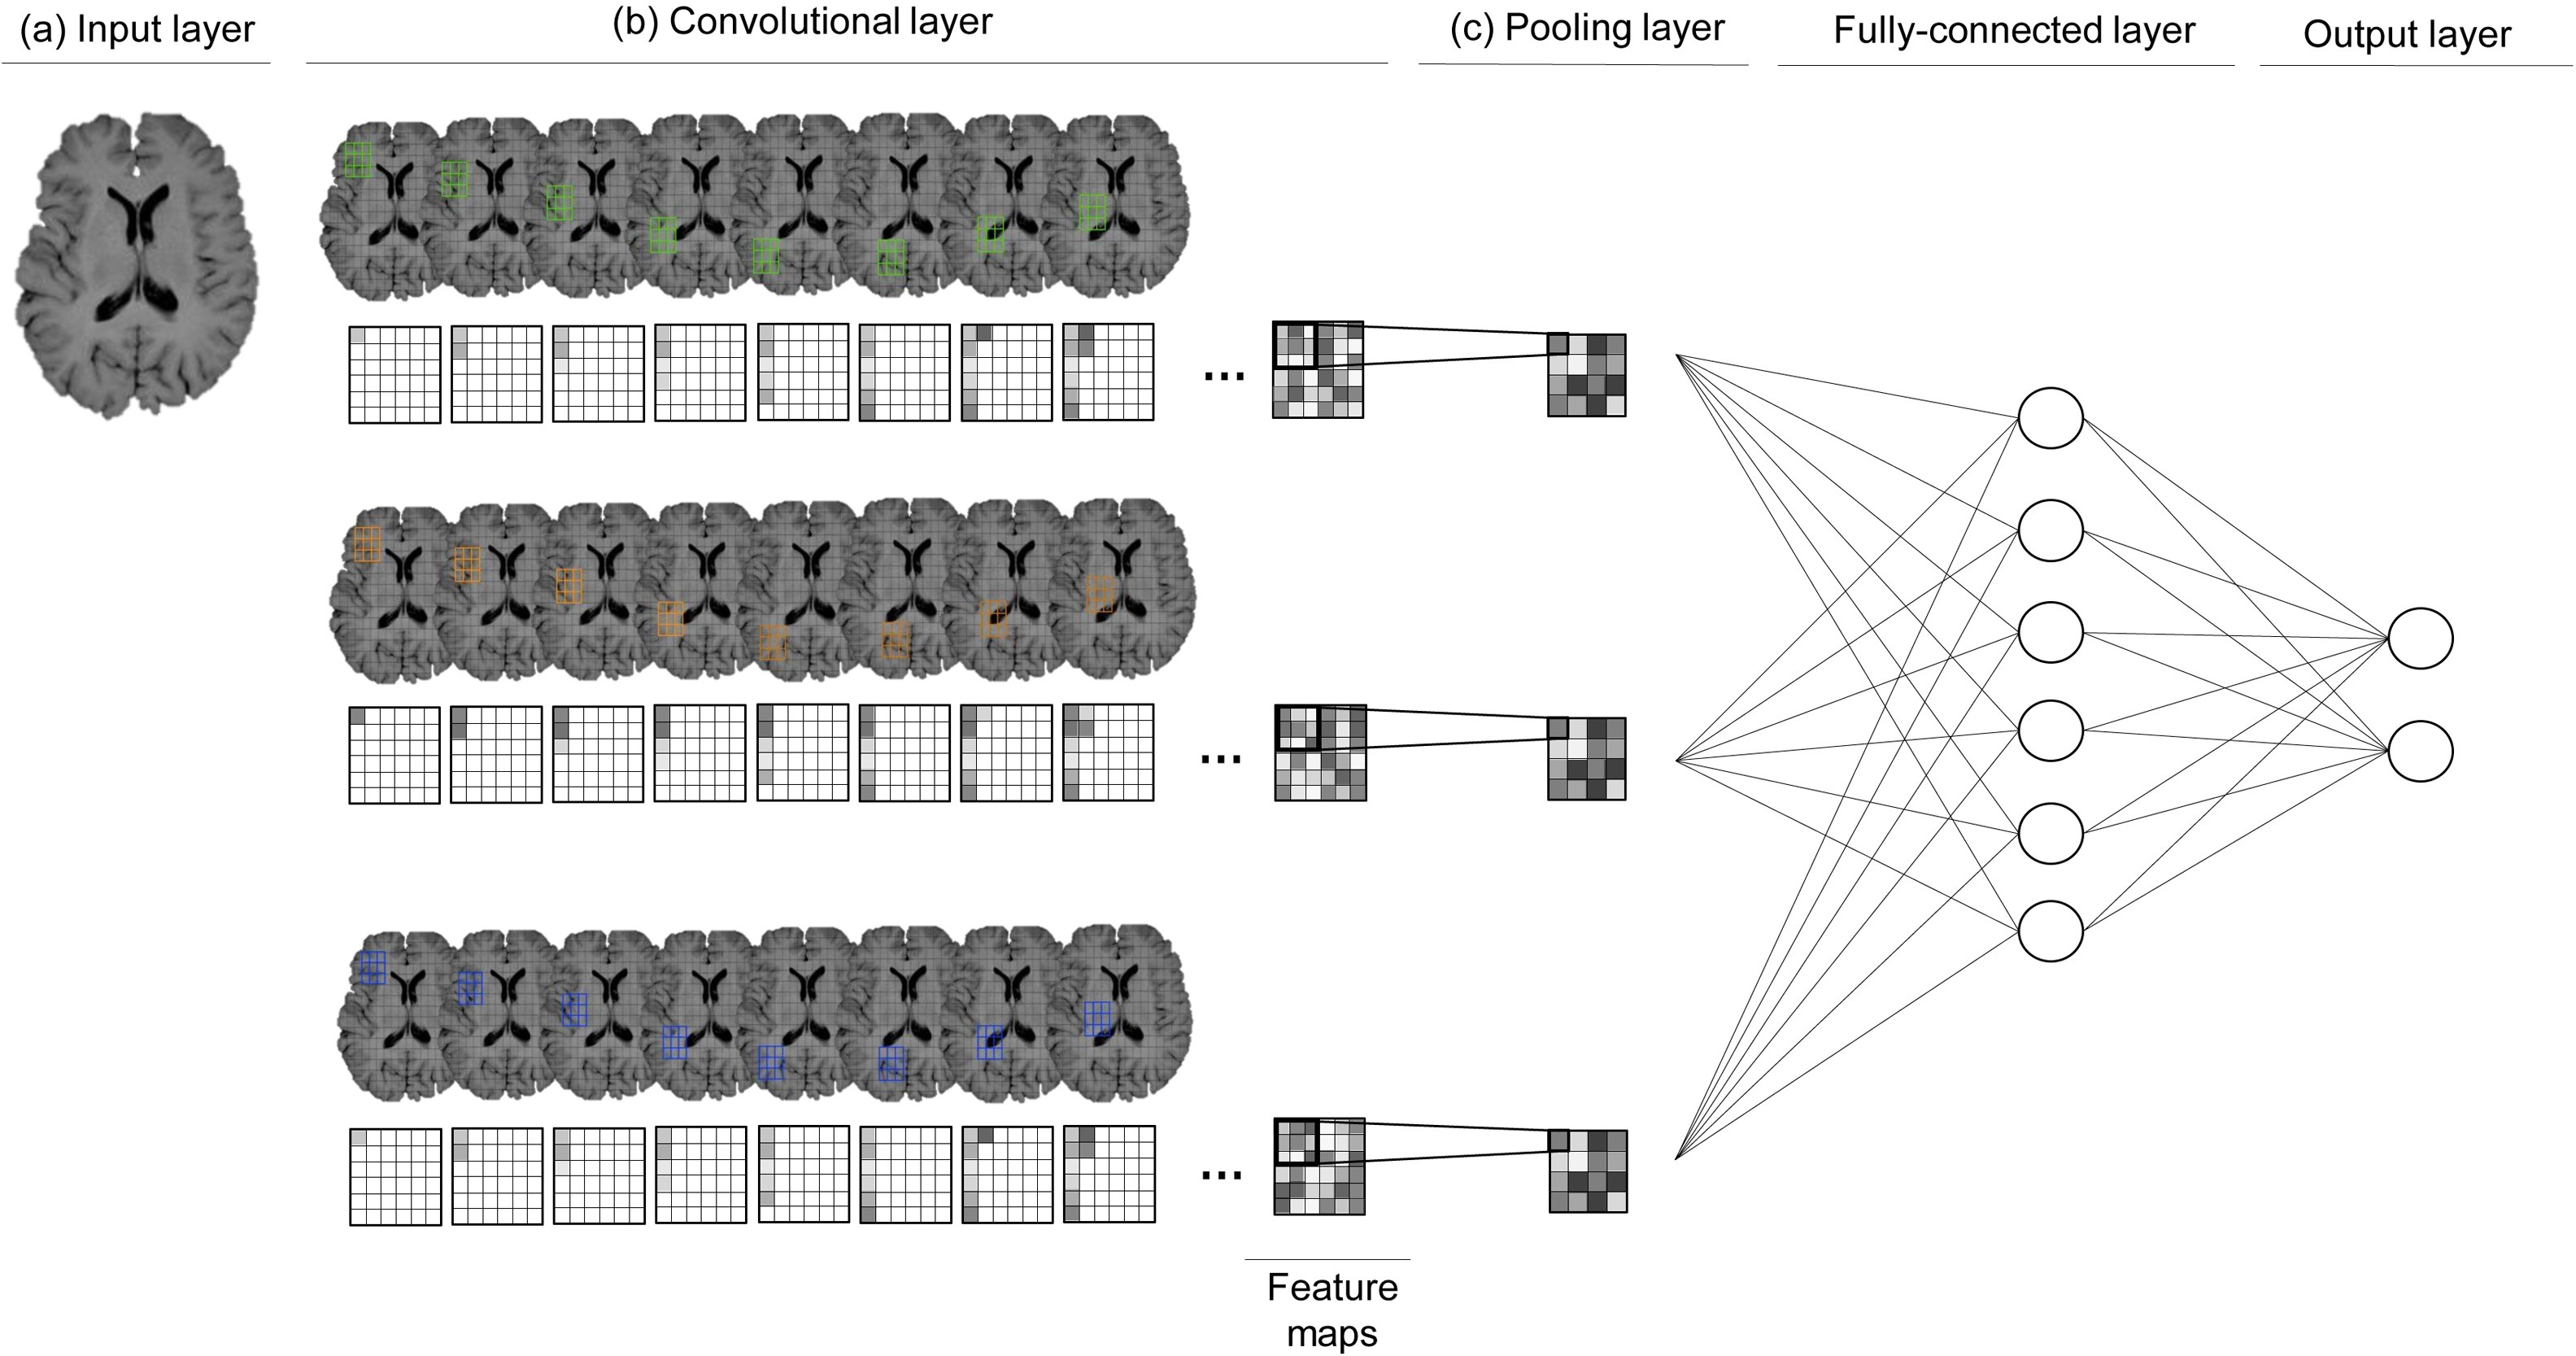
\includegraphics[scale=.9]{figures/DL.jpg}
        \caption[Simplified CNN architecture]{\footnotesize Simplified CNN architecture. Reprinted from \citetitle{vieiraUsingDeepLearning2017} by Vieira et al., \textit{Neuroscience & Biobehavioral Reviews}, 74, p.62. Copyright 1969 by Elsevier. }
    \label{fig:cnn}
\end{figure}
%%%%%%%%%%%%%%%%%%%%%%%%%%%%%%%%%%%%%%%%%%%%%%%%%%%%%%%
\newpage
\subsection{Bias-Variance Trade-off} \label{bias-variance}

Generalization is a fundamental goal of \gls{ML} techniques and refers to the idea of using a model that has been trained on a finite sample of observation to make accurate predictions about novel data \autocite{foundationof}. To assess a models generalizability, test error, that is the prediction error a model makes on novel data, is of importance. The two sources that produce to this error rate are termed \texif{bias} and \textif{variance} \autocite{westfall}. 
In \textcite{introtostat}, variance is described as to what extend the estimated true function learned by a statistical learning method would differ if estimated using different training data. So, for methods that have high variance, small changes in the training set could lead to more variety in the estimated function compared to method with low variance. Bias is described as the error that can happen while approximating complex relations with a simpler model. An example being a linear regression assuming linearity between variable that are likely to be non-linear and thus having some amount of bias in its estimation. Put differently, the bias of a model is a systematic tendency for its predictions to deviate from the true value \autocite{westfall}. Both variance and bias are connected and increasing one would decrease the other and therefore consideration have to be made on the optimum ratio of bias and variance \autocite{introtostat}. Over fitting for example occurs with low bias and high variance meaning that the model learns irrelevant patterns from the training set that are caused by random chance \autocite{introtostat}. Under fitting, on the other hand reflects model with high bias \autocite{deeplearningav}. Typically, methods that are more flexible have less bias but higher variance \autocite{introtostat}. 
In \gls{ML} choosing a ratio that minimizes the expected prediction error seems the clear goal if data sets are large, assessment of a model's performance can be made objectively and if the used model allows for some control over bias-variance trade-off \autocite{westfall}. 





%%%%%%%%%%%%%%%%%%%%%%%%%%%%%%%%%%%%%%%%%%%%%%%%%%


%%%%%%%%%%%%%%%%%%%%%%%%%%%%%%%%%%%%%%%%%%%%%%%%%%%%%
\subsection{Training Data} \label{Training Data}
Figure \ref{fig:workflow} shows the different steps involved in supervised machine learning. It follows a description of pre-processing step \ref{prep} and feature selection \ref{Input Data Management}. \gls{cnn} combines feature selection, feature vectors and classifier, whereas \gls{svm} is just a classifier. 

\begin{figure}[H]
    \centering
        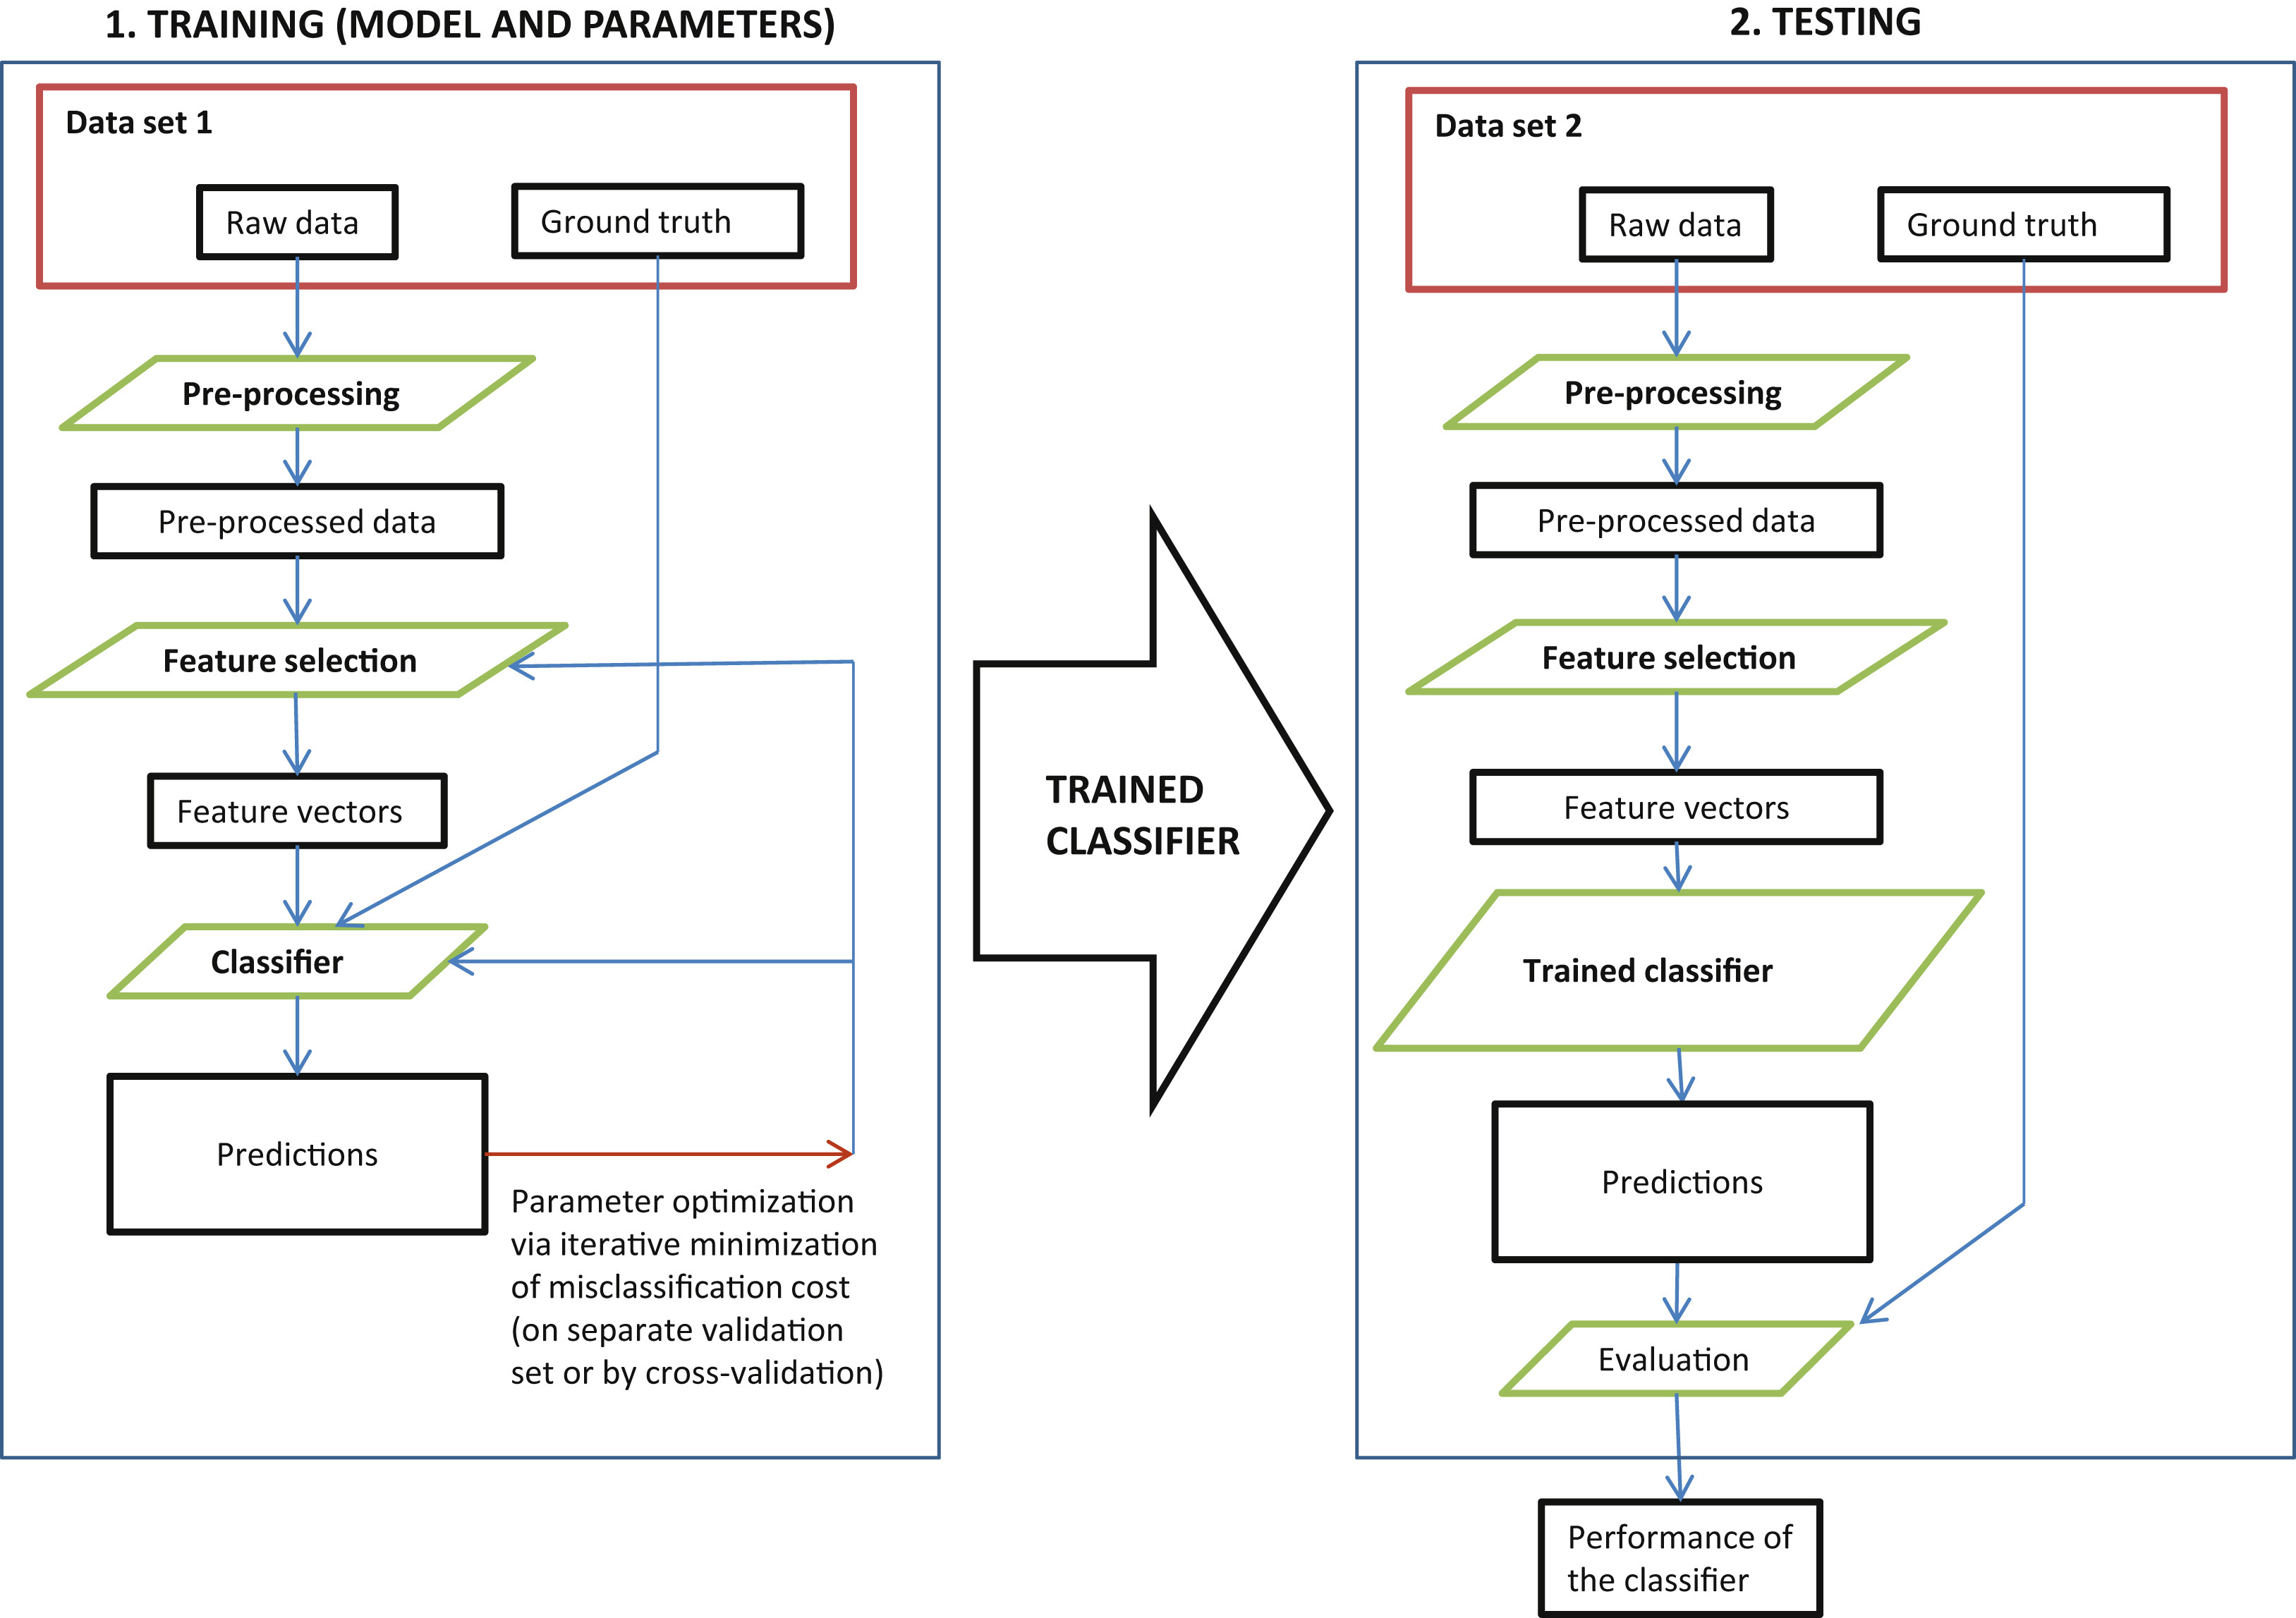
\includegraphics[scale=.9]{figures/gr1.jpg}
        \caption[Classification workflow for supervised learning]{\footnotesize Classification workflow for supervised learning. Reprinted from \citetitle{pellegriniMachineLearningNeuroimaging2018} by Pellegrini et al.,\textit{Alzheimers Dement}, 10, p.520. Copyright 2018 by the authors.}
    \label{fig:workflow}
\end{figure}

\subsubsection{Pre-processing} \label{prep}
A core problem with data is that it can be noisy (e.g. containing random and irrelevant information) \autocite{introdeep}. Pre-processing can help with reducing noise in data and is a important step in increasing the quality of input data \autocite{noorApplicationDeepLearning2020} with the hope of making it easier for the statistical learning method to find relevant patterns \autocite{bishop2006pattern}. A review by \textcite{ebrahimighahnaviehDeepLearningDetect2020} states that \gls{in}, \gls{ir} and \gls{sst} are among the most often used pre-processing techniques when using \gls{mri}-images for \gls{AD} classification. \gls{in} is a normalization technique that helps with comparison between \gls{mri} scans and does so by reducing the voxel or pixel intensity variation which can be caused if different scanners are used \autocite[as cited in][]{noorApplicationDeepLearning2020}. \gls{ir} is a second technique that helps with aligning the image scan to the anatomic brain structure so that a voxel position contains the same anatomical structure while comparing \gls{mri}-images of different people \autocite{ebrahimighahnaviehDeepLearningDetect2020}. \gls{sst} is done to remove the skull from MRI images \autocite{ebrahimighahnaviehDeepLearningDetect2020}.


\subsubsection{Input Data Management} \label{Input Data Management}
%Feature selection is a significant step in the classification process \autocite{tanveerMachineLearningTechniques2020}.

%There are different features that can be selected from \gls{mri} images. 
In a review \textcite{ebrahimighahnaviehDeepLearningDetect2020} found that voxel-based, slice-based, patch-based and \gls{roi} based approaches are used to manage the input data. 
The authors describe voxel-based as a method that uses the intensity values of every voxel in a given MRI scan as input, therefore using information of the full brain image. This approach, also sometimes referred to as subject-level approach has the advantage of including spatial information of the whole image but has the drawback of needing to optimize many parameters \autocite{wenConvolutionalNeuralNetworks2020}. Reducing feature dimensionality can help in this regards. For example, tissue segmentation can be done therefore only including the values of voxels belonging to a tissue component (e.g. grey or white matter) \autocite{ebrahimighahnaviehDeepLearningDetect2020}. Another approach is the slice-based that extracts a 2D image (i.e. a slice) from of the 3D \gls{mri} image. A further discussed approach is called patch-based  and reflects the idea of using three-dimensional cubes (i.e. a patches) to form a subset of voxels of the \gls{mri} image and are then used for feature extraction. \textcite{ebrahimighahnaviehDeepLearningDetect2020} point out that a challenge is to choose patches that contain all disease relevant information. \gls{roi}-based approach, on the other hand, uses prior knowledge about brain structures that are affected by the disease and a brain atlas to group voxels into relevant anatomical regions which are then used as input \autocite{ebrahimighahnaviehDeepLearningDetect2020}.

A further technique that some studies (e.g. \autocite{akramifardEmphasisLearningFeatures2020, syaifullahMachineLearningDiagnosis2021}) make use of is \gls{vbm} and can be seen as a voxel-based approach. \textcite{mechelliVoxelBasedMorphometryHuman2005} refer to \gls{vbm} as a mass uni-variate approach that performs voxel-based comparison between images to find significant differences. Normalisation, segmentation of white and gray matter and other pre-processing steps are done to help standardizing the images. Then, statistical analysis (e.g. t-tests and F-tests) find voxel-based differences. This approach can be used to pre-process the data or to find \gls{roi} \autocite[see][]{syaifullahMachineLearningDiagnosis2021, akramifardEmphasisLearningFeatures2020}. 


\subsubsection{Database} \label{database}

\gls{adni} is a study in which \textit{200} elderly \gls{nc}, \textit{400} with \gls{mci} and \textit{200} with \gls{AD} were followed three years while collecting multiple data such as \gls{MRI}, clinical/psychometric assessments, urine serum, \gls{pet}. The described aims of the study were to make the information available for the scientific community, standardizing imaging in longitudinal studies, finding optimal methods of analysing images and validating biomarkers \autocite{jack2008alzheimer}. \textcite{weiner2013alzheimer} state that since the start of \gls{adni} in North America in 2004, different studies worldwide have been done using the \gls{adni} protocols. For example, \gls{aibl} was a study done in Australia with a cohort of \textit{177} \gls{nc}, \textit{57} \gls{mci} and \textit{53} \gls{AD} subjects. Further, \gls{adni} studies have been done to extend the original cohort \autocite{weiner2013alzheimer} and is now in its third instalment \gls{adni}-3 \autocite{weiner2017alzheimer}.  
Other online databases that contain neuroimaging modalities are: \gls{oasis} \autocite{kurdi2017introducing} and \gls{miriad} \autocite{malone2013miriad}.
%%%%%%%%%%%%%%%%%%%%%%%%%%%%%%%%%%%%%


\subsection{Model Assessment and Model Selection} \label{Model Selection}
Model assessment refers to the evaluation of the model's performance \autocite{introtostat}. Accuracy, specificity and sensitivity are metrics that are used to analyse the performance of a \gls{ML} classification model \autocite{noorApplicationDeepLearning2020}. Accuracy is the most commonly used measurement to test the performance and consists of the fraction of correctly predicted classes in a test set \autocite{pereiraMachineLearningClassifiers2009}. Sensitivity and specificity as further measurements, are described by \textcite{noorApplicationDeepLearning2020}, as the percentage of true positives that have been predicted as such (sensitivity) and true negative cases that have been predicted correctly (specificity).
The term \textit{model selection}, on the other hand, is used for the process of selection a model's right flexibility \autocite{introtostat}. As mentioned in \ref{bias-variance}, choosing the right flexibility (e.g bias-variance trade-off) is important for \gls{ML} techniques.
\gls{cv}, as describe in \textcite{introtostat}, is a method that is used to help with model assessment and model selection. It does so by splitting the training data into a training set and a testing set whereas the model is fitted with the training set and afterwards its performance is evaluated on the testing set. With classification models the accuracy metric is used for evaluation. Furthermore \gls{loocv} is described as a variation of \gls{cv} where a single observation of the training data is left out for validation and the rest are used to train the model. This process is repeated as many times as there are observations in the training data (e.g. \textit{n}) while differing the observation that is used for validation. Essentially, \gls{loocv} produces \textit{n} different models that are fitted and validated with different training and testing sets. Averaging the \textit{n} accuracy rates that \gls{loocv} produce leads to a better estimation of the true error rate the model would have while confronted with novel data. 
\textcite{introtostat} name \gls{kfold} as second variation of \gls{cv}. K-fold CV randomly divides the training data into \textit{k} groups so that one group can be used for validation while \textit{k-1} groups train the model. This process is done \textit{k} times while changing the validation group. Finally, averaging the accuracy rates which results in an estimator for the true error rate. As \textcite{introtostat} point out if \textit{k} would be set to \textit{n}, than \gls{kfold} would be the same as \gls{loocv}.  

\newline












